\chapter{Image Processing}\label{ch:imageprocessing}

Now that we've covered all the basics of how to manipulate images, 
it's time to move on to some more interesting image processing 
tasks.  We begin with an introduction to image filtering, followed 
by a discussion of image math.  We then take a brief detour to 
introduce the Vision Workbench's \verb#Vector# and \verb#Matrix# 
classes before describing image transformation and warping.

By the end of this chapter you will have encountered all of the core
building blocks that comprise the heart of the Vision Workbench.
There are a number of directions that you can go from here, depending
on what you are hoping to accomplish.  We conclude this chapter with
an overview of the many more specialized features of the Vision
Workbench and a discussion of where to look (in this book and
elsewhere) in order to learn more about them.

\section{Image Filtering}

Image filtering has traditionally been the bread and butter of image
processing software packages.  The Vision Workbench includes a number
of functions to perform the most common filtering operations.  We will
first describe the special-purpose filters, and then we will discuss
the more general convolution-based linear filtering functions.  All of
the filter functions discussed in this section are defined in the
header file \verb#<vw/Image/Filter.h>#.  We will not discuss
frequency-domain filtering in this chapter; that is covered later in
Section~\ref{sec:advanced.frequency}.

\begin{table}[t]\begin{centering}
\begin{tabular}{|c|l|l|} \hline
Function & Description \\ \hline \hline
\verb#gaussian_filter(im,...)# & Apply a Gaussian smoothing filter to an image \\ \hline
\verb#derivative_filter(im,...)# & Apply a discrete differentiation filter to an image \\ \hline
\verb#laplacian_filter(im,...)# & Apply a discrete Laplacian filter to an image \\ \hline
\verb#convolution_filter(im,...)# & Apply a general 2D convolution filter to an image \\ \hline
\verb#separable_convolution_filter(im,...)# & Apply a separable convolution filter to an image \\ \hline
\end{tabular}
\caption{The Vision Workbench image filtering functions, defined in {\tt <vw/Image/Filter.h>}.}
\label{tbl:image-filters}
\end{centering}\end{table}

\subsection{The Special-Purpose Filters}

At the moment only three special-purpose filters are fully supported.
The first is a Gaussian smoothing or blurring filter, which convolves
the image with a discrete Gaussian kernel that has a user-specified
standard deviation (a.k.a. ``sigma'') and user-specified size in each
axis. In order for the filter to accurately approximate a Gaussian,
the size of the kernel should be at least a few times the standard
deviation.  However, unnecessary computation is performed if the size
is much larger than that.  You can omit the size arguments, in which
case the function will pick a kernel size based on your standard
deviation that is reasonable for most applications.  In the most
common case the two standard deviations are equal, in which case you
need only specify a single value for sigma.
\begin{verbatim}
  result = gaussian_filter( image, sigma );
  result = gaussian_filter( image, xsigma, ysigma );
  result = gaussian_filter( image, xsigma, ysigma, xsize, ysize );
\end{verbatim}
In these examples, the \verb#sigma# arguments are generally
floating-point whereas the \verb#size# variables are integers.

The next filter is the derivative filter, which performs a 
discrete spatial differentiation of your image.  Here again, you 
can specify the order of differentiation in the two axes as well 
as the filter kernel size.
\begin{verbatim}
  result = derivative_filter( image, xderiv, yderiv );
  result = derivative_filter( image, xderiv, yderiv, xsize, ysize );
\end{verbatim}
There is a minimum filter size below which it is not possible compute
any given derivative, and these functions will throw an exception if
you try.  For the most part it is a good idea to just let the Vision
Workbench pick the kernel size.

The final special-purpose filter is the Laplacian filter, which 
performs a discrete approximation to the Laplacian operation
$\nabla^2=\frac{d^2}{dx^2}+\frac{d^2}{dy^2}$.
\begin{verbatim}
  result = laplacian_filter( image );
\end{verbatim}
This filter does not take any special parameters.  Note that if you 
are accustomed to using a ``larger'' derivative or Laplacian filter 
to reduce the effect of noise, you are probably better off applying 
a smoothing operation (e.g. via \verb#gaussian_filter()#) first.

\subsection{Edge Extension Modes}
\label{sec:filter-edge-extend}

\begin{table}[t]\begin{centering}
\begin{tabular}{|c|l|l|} \hline
Type & Description \\ \hline \hline
\verb#ConstantEdgeExtension# & Extends an image with constant (i.e. nearest-neighbor) values \\ \hline
\verb#ZeroEdgeExtension# & Extends an image with a zero value in all directions \\ \hline
\verb#ReflectEdgeExtension# & Extends an image by reflecting across its edges \\ \hline
\verb#PeriodicEdgeExtension# & Extends an image by repeating it periodically \\ \hline
\end{tabular}
\caption{The edge extension modes.}
\label{tbl:edge-extension-modes}
\end{centering}\end{table}

To filter the regions near the edges of an image properly, 
filters like these need to make some sort of assumption 
about the contents of the source image {\it beyond} the 
image boundaries.  This is generally referred to as ``edge 
extension''.  The default assumption made by the filters 
discussed in this section is that in each direction the 
image is extended with a constant value equal to the value 
of the nearest edge pixel.  However, you can specify an 
alternative edge extension mode if you wish, by passing 
an extra argument to the filters.  The C++ type of the 
argument determines the edge extension mode used.  
\begin{verbatim}
  result = gaussian_filter( image, 3.0, ConstantEdgeExtension() );
  result = gaussian_filter( image, 3.0, ZeroEdgeExtension() );
\end{verbatim}
Both of these examples filter the source image using a 
standard deviation of three pixels and an automatically-chosen 
kernel size.  However, the first explicitly requests the 
default edge extension behavior, while the second requests 
that the source image be assumed to be zero outside the 
image boundaries.

Notice the ``extra'' set of parentheses after the names 
of the edge extension modes.  Remember that those names are 
C++ {\it types}, and you can only pass an {\it object} as an 
argument to a function.  Those parentheses invoke the 
edge extension type's constructor, returning a dummy 
object that you pass as the final argument to the filtering 
function.  If you find this confusing, don't worry too much 
about it right now.  Just keep in mind that when you're 
using a type as an argument to a function to change its 
behavior you need the extra parentheses.  The types that 
are currently supported as edge extension modes are listed 
in Table~\ref{tbl:edge-extension-modes}.

\subsection{General Convolution Filtering}

Most of the filters used in image processing are convolution filters,
which express each output pixel as a fixed weighted sum of neighboring
input pixels.  An image convolution filter is usually described by a
rectangular array of weights called the {\it kernel}.  The easiest way
to think about an image kernel is as the result that you would desire 
from the filter if the input image had the value $1$ at the origin and
zero everywhere else.  (This is also known as the ``impulse response''
of the filter.)  For example, a first-order derivative filter in the
$x$ direction might have the kernel
$[\begin{array}{ccc} 1 & 0 & -1 \end{array}]$.
In this case we also need to know that the middle number of the kernel 
(the zero in this case) is the kernel's origin.

In the Vision Workbench, convolution kernels---which as we've said are 
nothing more than rectangular arrays of numbers---are represented by 
images.  The pixel type for a kernel should generally be a scalar type 
such as \verb#float#.  Once you've put the kernel that you'd like into 
an image it is straightforward to use it to filter another image.
\begin{verbatim}
  ImageView<float> kernel;
  /* set up your kernel here */
  result = convolution_filter( image, kernel );
\end{verbatim}
In this case the Vision Workbench assumes that the center pixel of the
kernel is the kernel's origin.  If this is not what you want then you
can specify the coordinates of the kernel's origin explicitly instead.
\begin{verbatim}
  result = convolution_filter( image, kernel, ox, oy );
\end{verbatim}
In either case you can also optionally specify an edge extension mode, 
just like you could for the special-purpose filters.

Convolution filtering can be computationally expensive if the kernel
is large.  Fortunately, many useful kernels have a special form that
makes it possible to improve the performance considerably.  These are
called {\it separable} kernels, and are themselves the result of
convolving a single-column image with a single-row image.  In other
words, the kernel $K$ must satisfy $K(x,y)=K_x(x)K_y(y)$ for some
functions $K_x$ and $K_y$.  The Gaussian and derivative filters
are both of this form, for example, though the Laplacian filter is
not.

The Vision Workbench provides special support for efficient 
convolution filtering with separable kernels.  You must supply the 
{\it separated} kernel, i.e. two one-dimensional kernels.
\begin{verbatim}
  result = separable_convolution_filter( image, xkernel, ykernel );
  result = separable_convolution_filter( image, xkernel, ykernel, ox, oy );
\end{verbatim}
As in the general 2D convolution case, the origin of the kernel is 
assumed to be in the middle if you do not specify otherwise and in 
either case you can add an optional argument specifying the edge 
extension mode.  You can still supply the one-dimensional kernels as 
images, just as you did in the general 2D convolution case, but here 
you can also provide them in another STL-compliant container, such 
as a \verb#std::vector# or (as we shall introduce later this chapter) 
a \verb#vw::Vector#.  If you do chose to represent the kernels as 
images, remember that each should have one of the dimensions set to 1.

\section{Doing Math with Images}

In image processing it is often desirable to perform some mathematical 
operation on every pixel of an image, or to corresponding pixels from 
several images.  For example gamma correction involves applying a 
mathematical function to each pixel, and background subtraction involves
subtracting the corresponding pixels from two images.  In the Vision 
Workbench, these operations and others like them fall under the rubric 
of ``image math'', and the functions to support them are defined in the 
header \verb#<vw/Image/ImageMath.h>#.

\subsection{Image Operators}

In most cases writing code to perform image math is trivial.  The 
mathematical expressions that you would normally write for individual 
pixels work just as well for whole images of pixels.  For example, 
consider the background subtraction problem mentioned above.
\begin{verbatim}
  result_image = input_image - background_image;
\end{verbatim}
That's all there is to it.  Setting up an IIR low-pass filter to 
estimate the background image is just as easy.
\begin{verbatim}
  background_image = alpha*input_image + (1-alpha)*background_image;
\end{verbatim}
(Here we're assuming that \verb#alpha# is a small positive
floating-point number.)  The important point is that there is no need
for you to write a loop that performs an operation like this on each
pixel.  Just write the mathematical expression, replacing pixels with
images, and you're all set.

\begin{table}[t]\begin{centering}
\begin{tabular}{|c|c|c|c|} \hline
Per-pixel Sum & Per-pixel Difference & Per-pixel Product & Per-pixel Quotient \\ \hline \hline
\verb#image + image#  & \verb#image - image#  & \verb#image * image#  & \verb#image / image#  \\ \hline
\verb#image += image# & \verb#image -= image# & \verb#image *= image# & \verb#image /= image# \\ \hline
\verb#image + value#  & \verb#image - value#  & \verb#image * value#  & \verb#image / value#  \\ \hline
\verb#image += value# & \verb#image -= value# & \verb#image *= value# & \verb#image /= value# \\ \hline
\verb#value + image#  & \verb#value - image#  & \verb#value * image#  & \verb#value / image#  \\ \hline
\end{tabular}
\caption{The Vision Workbench image operators are included
  automatically when you include {\tt <vw/Image/ImageMath.h>}).}
\label{tbl:image-operators}
\end{centering}\end{table}

This works, of course, because the Vision Workbench has overloaded the
standard C++ mathematical operators to work on images.  These
operators are listed in Table~\ref{tbl:image-operators}.  Operation
with scalars is treated identically to per-pixel operation with
constant-value images.  In order to simplify division with large
images, the image division operators have been designed so that
division by zero returns zero instead of throwing an exception.

There is one important issue to bear in mind when using image
operators: the underlying per-pixel operations must themselves be
meaningful.  For example, multiplying an image whose pixel type is
\verb#PixelGray# by an image whose pixel type is \verb#PixelRGB# is
not well-defined, and attempting to do so will result in a compiler
error.  The Vision Workbench will not automatically ``promote'' the
grayscale image to RGB.

This raises the question of what happens when you multiply two images
both of whose pixel type is, for example, \verb#PixelRGB#.  What does
it mean to multiply two RGB colors?  Multiplication is defined for
numbers, not colors.  The answer is that in this situation the Vision
Workbench will actually perform the mathematical operation on a
per-{\it channel} basis rather than just a per-pixel basis.

A good rule of thumb when working with image operators is to restrict
yourself to operating on images of the same type, or combinations of
images of one type and images of scalars.  As long as you obey this
rule you should find that the image operators always do what you
expect.

\subsection{Mathematical Functions}

\begin{table}[t]\begin{centering}
\renewcommand\arraystretch{1.2}
\begin{tabular}{|c|c|c|c|} \hline
Function & Description & Function & Description \\ \hline \hline
\verb#sin# & Sine, $\sin x$ & \verb#asin# & Inverse sine, $\sin^{-1} x$ \\ \hline
\verb#cos# & Cosine, $\cos x$ & \verb#acos# & Inverse cosine, $\cos^{-1} x$ \\ \hline
\verb#tan# & Tangent, $\tan x$ & \verb#atan# & Inverse tangent, $\tan^{-1} x$ \\ \hline
\verb#atan2# & \multicolumn{3}{|l|}{Two-argument form of inverse tangent, $\tan^{-1}\!\!\ ^x\!/\!_y$ } \\ \hline
\verb#sinh# & Hyperbolic sine, $\sinh x$ & \verb#cosh# & Hyperbolic cosine, $\cosh x$ \\ \hline
\verb#tanh# & Hyperbolic tangent, $\tanh x$ & \verb#exp# & Exponential, $e^x$ \\ \hline
\verb#log# & Natural logarithm, $\ln x$ & \verb#log10# & Base-10 logarithm, $\log_{10} x$ \\ \hline
\verb#ceil# & Ceiling function, $\lceil x \rceil$ & \verb#floor# & Floor function, $\lfloor x \rfloor$ \\ \hline
\verb#sqrt# & Square root, $\sqrt{x}$ & \verb#pow# & Power function, $x^y$ \\ \hline
\hline
\verb#asinh# & Inverse hyperbolic sine, $\sinh^{-1} x$ & \verb#acosh# & Inverse hyperbolic cosine, $\cosh^{-1} x$ \\ \hline
\verb#atanh# & Inverse hyberbolic tangent, $\tanh^{-1} x$ & \verb#cbrt# & Cube root, $\sqrt[3]{x}$ \\ \hline
\verb#exp2# & Base-2 exponential, $2^x$ & \verb#expm1# & Exponential minus 1, $e^x-1$ \\ \hline
\verb#log2# & Base-2 logarithm, $\log_2 x$ & \verb#log1p# & Lograithm of one-plus, $\ln (1+x)$ \\ \hline
\verb#tgamma# & Gamma function, $\Gamma(x)$ & \verb#lgamma# & Log of Gamma function, $\ln |\Gamma(x)|$ \\ \hline
\verb#hypot# & Hypotenuse, $\sqrt{x^2+y^2}$ & \verb#copysign# & Sign-copying function \\ \hline
\verb#round# & Rounding function & \verb#trunc# & Floating-point truncation \\ \hline
\verb#fdim# & Positive difference, $\max(x-y,0)$ & & \\ \hline
\end{tabular}
\caption{The Vision Workbench image math functions, as defined in {\tt <vw/Image/ImageMath.h>}.
The functions in the bottom section are not available under the Windows operating system.}
\label{tbl:math-functions}
\end{centering}\end{table}

Of course, C++ provides a range of mathematical functions, too, such
as exponentials and logarithms, trigonometric functions, and so forth.
The Vision Workbench extends these functions to operate on images as
well.  The supported functions are listed in
Table~\ref{tbl:math-functions}.  Note that these image functions are
built on top of the standard C++ functions that operate on regular
numbers.  Therefore, the Vision Workbench only supports those
functions that are provided by your platform.  In particular, the
bottom half of Table~\ref{tbl:math-functions} lists functions that are
{\it not} currently available under the Microsoft Windows operating
system.

You can use these functions just like you use the mathematical 
operators: write the same expression that you would write for 
individual pixels, but substitute whole images instead.
\begin{verbatim}
  float gamma = 1.8;
  result_image = pow( input_image, gamma );
\end{verbatim}
This example demonstrates how to use the \verb#pow()# function to
gamma-correct an image.  Here the variable \verb#gamma# is a
floating-point number representing the desired gamma correction factor
for the entire image.  However, if instead we wanted to apply a variable
gamma correction factor on a per-pixel basis, the following code would
do the trick.
\begin{verbatim}
  ImageView<float> gamma_image; // Initialize with different gamma values
  result_image = pow( input_image, gamma_image );
\end{verbatim}
This example demonstrates that the arguments of a two-argument
mathematical function can be either scalar or image values.  Just as
with the operators, scalar arguments are treated the just like a
constant-value image.

Note that unlike the normal mathematical functions that C++ inherited
from C, it is not necessary (or correct) to use a different function
name when you are working with \verb#float# image data than you would
use to work with \verb#double# image data.  The function names listed
in Table~\ref{tbl:math-functions} are correct for image math in all
cases.  Those in turn use the proper underlying mathematical functions
as appropriate---for example, \verb#sin()# invokes \verb#sinf()# on 
each pixel if it is applied to a \verb#float#-based image.

\section{Vectors and Matrices}

Before introducing the next image processing topic, image transformation 
and warping, we must first take a brief detour to introduce the Vision 
Workbench vector and matrix classes.  We will assume in this chapter 
that you have a good familiarity with the underlying mathematical 
entities that these classes represent.  Note that our mathematical usage 
of the word ``vector'' here is somewhat different from the C++ standard 
library's use of the word to mean a dynamically-resizable array.

\subsection{Vectors and Vector Operations}

The Vision workbench vector class is called, appropriately enough, 
\verb#Vector#.  Like \verb#ImageView#, \verb#Vector# is a template 
class whose first template parameter is required and specifies the 
underlying numeric type.  However, while the dimensions of an image 
are always specified at run-time via the image's constructor or the 
\verb#set_size()# method, \verb#Vector# comes in two variants.  The 
first form behaves in just the same way, but the second form has a 
fixed size that is specified at compile time.  This eliminates the 
need for frequent dynamic allocation when working with vectors in 
the common case when the vector dimension is known.

Declaring either type of vector is straightforward:
\begin{verbatim}
  Vector<float> vector1(3);
  Vector<float,3> vector2;
\end{verbatim}
Both of those statements declare three-dimensional vectors of 
floating-point numbers.  In the first case the vector is allocated 
dynamically on the heap and the size could have been chosen at 
run-time.  In the second case the vector is allocated statically 
on the stack, but the dimension can {\it not} vary at run time.
The first form is generally useful when, say, reading a large 
vector of data in from a file, while the second form is more 
useful when performing geometric computations.

The second, fixed-dimension form also has special constructors that
you can use to initialize the vector contents:
\begin{verbatim}
  Vector<float,3> vector2(1,2,3);
\end{verbatim}
These constructors are available with up to four arguments.
Alternatively, you can construct both fixed-size and dynamically-sized 
vector with data copied from a block of memory that you point them to:
\begin{verbatim}
  float *some_data;
  Vector<float> vector1(3, some_data);
  Vector<float,3> vector2(some_data);
\end{verbatim}
Remember that this copies the data, so it can be inefficient; see 
the discussion of \verb#VectorProxy# below for an alternative.
Three of the most commonly used vector types have special aliases, 
for convenience:
\begin{verbatim}
  typedef Vector<double,2> Vector2;
  typedef Vector<double,3> Vector3;
  typedef Vector<double,4> Vector4;
\end{verbatim}
These types are used throughout the Vision Workbench as the standard
geometric vector types.

You can query a vector about its size (i.e. dimension or length) with
the \verb#size()# method, and you can index into a vector to access 
individual elements:
\begin{verbatim}
  for( unsigned i=0; i<vector1.size(); ++i ) vector1(i) = 0;
\end{verbatim}
This example loops over all the elements of a vector, setting them 
to zero.  You can also into a vector with square brackets instead 
of parentheses if you prefer.  For fixed-length vectors there is one 
more way to access up to the first three elements, via methods called 
\verb#x()#, \verb#y()#, and \verb#z()#.
\begin{verbatim}
  vector2.x() = 0;  // Set the first element to zero
\end{verbatim}
These methods are only available if the vector has sufficient 
length.  For example, attempting to use the \verb#z()# method of 
a vector of type \verb#Vector<float,2># will result in a compile-time 
error.  Remember, these methods are only available for fixed-size 
vectors, {\it not} dynamically-sized ones.  Dynamically-sized 
vectors, however, can be resized:
\begin{verbatim}
  vector1.set_size(10);
\end{verbatim}
The \verb#set_size()# function takes an optional second argument that 
specifies whether or not the vector contents should be preserved.  
This argument defaults to \verb#false#, so in the above example 
the old contents (if any) are lost.

\begin{table}[t!]\begin{centering}
\begin{tabular}{|c|l|} \hline
Function & Description \\ \hline \hline
\verb#- vector# & Vector negation \\ \hline
\verb#vector + vector# & Vector sum \\ \hline
\verb#vector - vector# & Vector difference \\ \hline
\verb#vector * scalar# & Scalar product \\ \hline
\verb#scalar * vector# & Scalar product \\ \hline
\verb#vector / scalar# & Scalar quotient \\ \hline
\verb#vector += vector# & Vector sum assignment \\ \hline
\verb#vector -= vector# & Vector difference assignment \\ \hline
\verb#vector *= scalar# & Scalar product assignment \\ \hline
\verb#vector /= scalar# & Scalar quotient assignment \\ \hline
\hline
\verb#elem_sum(vector,vector)# & Elementwise vector sum (same as \verb#+# operator) \\ \hline
\verb#elem_sum(vector,scalar)# & Elementwise sum of a vector and a scalar \\ \hline
\verb#elem_sum(scalar,vector)# & Elementwise sum of a scalar and a vector \\ \hline
\verb#elem_diff(vector,vector)# & Elementwise vector difference (same as \verb#-# operator) \\ \hline
\verb#elem_diff(vector,scalar)# & Elementwise difference of a vector and a scalar \\ \hline
\verb#elem_diff(scalar,vector)# & Elementwise difference of a scalar and a vector \\ \hline
\verb#elem_prod(vector,vector)# & Elementwise product of two vectors \\ \hline
\verb#elem_prod(vector,scalar)# & Elementwise vector product (same as \verb#*# operator) \\ \hline
\verb#elem_prod(scalar,vector)# & Elementwise vector product (same as \verb#*# operator) \\ \hline
\verb#elem_quot(vector,vector)# & Elementwise quotient of two vectors \\ \hline
\verb#elem_quot(vector,scalar)# & Elementwise quotient (same as \verb#/# operator) \\ \hline
\verb#elem_quot(scalar,vector)# & Elementwise quotient of a scalar and a vector \\ \hline
\hline
\verb#norm_1(vector)# & 1-norm of a vector, i.e. $\sum |v_i|$ \\ \hline
\verb#norm_2(vector)# & Euclidean 2-norm of a vector, i.e. $\sqrt{\sum v_i^2}$ \\ \hline
\verb#norm_2_sqr(vector)# & Squared 2-norm of a vector, i.e. $\sum v_i^2$ \\ \hline
\verb#norm_inf(vector)# & Infinity-norm of a vector, i.e. $\max |v_i|$ \\ \hline
\verb#sum(vector)# & Sum of elements, i.e. $\sum v_i$ \\ \hline
\verb#prod(vector)# & Product of elements, i.e. $\prod v_i$ \\ \hline
\verb#normalize(vector)# & The normalized form of a vector, i.e. $v/|v|$ \\ \hline
\verb#dot_prod(vector,vector)# & Vector dot product, i.e. $u\cdot v$ \\ \hline
\verb#cross_prod(vector,vector)# & Vector cross product, i.e. $u\times v$ \\ \hline
\end{tabular}
\caption{The vector math functions defined in {\tt <vw/Math/Vector.h>}.}
\label{tbl:vector-functions}
\end{centering}\end{table}

The \verb#Vector# classes support the standard mathematical operations
of vector addition and subtraction and scalar multiplication and
division via the usual C++ operators.  They also support the a range
of elementwise mathematical operations, such as adding a scalar to
each element or multiplying the corresponding elements of two vectors,
via functions of the form \verb#elem_*#.  There are a number of vector
norms and related functions, as well as a vector dot product and cross
product.  (The cross product is, of course, only valid for
three-dimensional vectors.)  The complete list of vector math
functions defined in \verb#<vw/Math/Vector.h># is given in
Table~\ref{tbl:vector-functions}.

A \verb#Vector# object is also a {\em container} in the C++ Standard Template 
Library sense of the word.  There is a \verb#Vector<...>::iterator# type 
that serves as the vector's iterator, and there are \verb#begin()# and 
\verb#end()# methods that return iterators to the first and one-past-the-last 
elements, as usual.  This can be an extremely convenient way to load 
data into and out of \verb#Vector#s.

You can extract a portion of a vector using the \verb#subvector()#
function, which takes three arguments: the original vector, the
position of the first element to extract, and the number of elements
in the resulting vector:
\begin{verbatim}
  Vector<float,3> vector2 = subvector(vector1,5,3);
\end{verbatim}
This example copies the fifth, sixth, and seventh elements of
\verb#vector1# into a new three-element vector.

The streaming operator \verb#<<# is also defined for writing vectors
to C++ output streams, which you can use to dump vector contents for
debugging:
\begin{verbatim}
  Vector<float,3> vector2(1,2,3);
  std::cout << vector2 << std::endl;
  // The output is: [3](1,2,3)
\end{verbatim}
Note that the size of the vector is printed first, followed by the 
vector's contents.

Sometimes it can be useful to work with data that is already stored in 
memory as though it were stored in a \verb#Vector# object.  As long as 
the data is stored in the usual packed format this is easy to do using 
the special \verb#VectorProxy# type, which also comes in fixed-size 
and dynamically-sized variants:
\begin{verbatim}
  float some_data[10] = {0,1,2,3,4,5,6,7,8,9};
  VectorProxy<float> proxy1(10, some_data);
  VectorProxy<float,10> proxy2(some_data);
\end{verbatim}
The constructor arguments are the same as are used in \verb#Vector# to
initialize a vector with data from a block of memory, except the data
is not copied.  You can now treat these proxy objects just like the
were regular \verb#Vector#s, except the contents will be stored in the
region of memory that you pointed them to.  In some situations this
can be considerably more efficient than copying the data
unnecessarily. (It is of course not possible to resize a
\verb#VectorProxy#, since the proxy does not have any control over the
memory that it is using.)

\subsection{Matrices and Matrix Operations}

The Vision Workbench \verb#Matrix# class is the matrix 
counterpart to the \verb#Vector# class, and behaves quite 
similarly.  Once again, there are fixed-dimension and 
dynamically-sized versions:
\begin{verbatim}
  Matrix<float> matrix1(3,3);
  Matrix<float,3,3> matrix2;
\end{verbatim}
Note that the arguments to matrix-related functions such 
as these constructors are given in $i,j$ order, i.e. row 
followed by column.  This is {\it different} from images, 
where arguments are given in $x,y$ order, i.e. column 
followed by row.  You may find this confusing at first if 
you are moving to the Vision Workbench from an environment 
like Matlab where there is no distinction between images 
and matrices.  However, it is in keeping with the standard 
index ordering seen in the bulk of the image processing 
and mathematics literatures, respectively.

You can initialize the matrix with data already stored 
in memory, as long as the data is stored in a packed 
row-major format:
\begin{verbatim}
  float some_data[4] = {1,2,3,4};
  Matrix<float> matrix1(2,2,some_data);
  Matrix<float,2,2> matrix2(some_data);
\end{verbatim}
As in the case of \verb#Vector#, the initialization data 
is {\it copied} into the matrix in this case, but there is 
also a proxy form that allows you treat in-memory data 
like an ordinary matrix:
\begin{verbatim}
  float some_data[4] = {1,2,3,4};
  MatrixProxy<float> matrix1(2,2,some_data);
  MatrixProxy<float,2,2> matrix2(some_data);
\end{verbatim}
The three most common matrix types have been given 
convenient aliases:
\begin{verbatim}
  typedef Matrix<double,2,2> Matrix2x2;
  typedef Matrix<double,3,3> Matrix3x3;
  typedef Matrix<double,4,4> Matrix4x4;
\end{verbatim}
These types are again the standard types used throughout the Vision 
Workbench in geometric applications.

You can query a matrix's dimensions using the \verb#rows()# and 
\verb#cols()# methods, and can index into the matrix to access 
individual elements.  There are two ways to do this:
\begin{verbatim}
  matrix(row,col) = 1;    // "New"-style indexing
  matrix[row][col] = 1;   // "Old"-style indexing
\end{verbatim}
A dynamically-sized matrix can be resized using the 
\verb#set_size()# method:
\begin{verbatim}
  matrix.set_size(rows,cols);
\end{verbatim}
As in the case of resizing vectors, the default behavior is that any
old data is not saved.  The \verb#set_size()# method takes an optional
third boolean parameter that can be set to \verb#true# to request that
it preserve the overlapping entries.

\begin{table}[t!]\begin{centering}
\begin{tabular}{|c|l|} \hline
Function & Description \\ \hline \hline
\verb#- matrix# & Matrix negation \\ \hline
\verb#matrix + matrix# & Matrix sum \\ \hline
\verb#matrix - matrix# & Matrix difference \\ \hline
\verb#matrix * scalar# & Scalar product \\ \hline
\verb#scalar * matrix# & Scalar product \\ \hline
\verb#matrix / scalar# & Scalar quotient \\ \hline
\verb#matrix += matrix# & Matrix sum assignment \\ \hline
\verb#matrix -= matrix# & Matrix difference assignment \\ \hline
\verb#matrix *= scalar# & Scalar product assignment \\ \hline
\verb#matrix /= scalar# & Scalar quotient assignment \\ \hline
\hline
\verb#matrix * matrix# & Matrix product \\ \hline
\verb#matrix * vector# & Matrix-vector product \\ \hline
\verb#vector * matrix# & Vector-matrix product \\ \hline
\hline
\verb#elem_sum(matrix,matrix)# & Elementwise matrix sum (same as \verb#+# operator) \\ \hline
\verb#elem_sum(matrix,scalar)# & Elementwise sum of a matrix and a scalar \\ \hline
\verb#elem_sum(scalar,matrix)# & Elementwise sum of a scalar and a matrix \\ \hline
\verb#elem_diff(matrix,matrix)# & Elementwise matrix difference (same as \verb#-# operator) \\ \hline
\verb#elem_diff(matrix,scalar)# & Elementwise difference of a matrix and a scalar \\ \hline
\verb#elem_diff(scalar,matrix)# & Elementwise difference of a scalar and a matrix \\ \hline
\verb#elem_prod(matrix,matrix)# & Elementwise product of two matrices \\ \hline
\verb#elem_prod(matrix,scalar)# & Elementwise matrix product (same as \verb#*# operator) \\ \hline
\verb#elem_prod(scalar,matrix)# & Elementwise matrix product (same as \verb#*# operator) \\ \hline
\verb#elem_quot(matrix,matrix)# & Elementwise quotient of two matrixs \\ \hline
\verb#elem_quot(matrix,scalar)# & Elementwise quotient (same as \verb#/# operator) \\ \hline
\verb#elem_quot(scalar,matrix)# & Elementwise quotient of a scalar and a matrix \\ \hline
\hline
\verb#norm_1(matrix)# & Matrix 1-norm \\ \hline
\verb#norm_2(matrix)# & Matrix 2-norm \\ \hline
\verb#norm_frobenius(matrix)# & Matrix Frobenius norm \\ \hline
\verb#sum(matrix)# & Sum of elements, i.e. $\sum v_i$ \\ \hline
\verb#prod(matrix)# & Product of elements, i.e. $\prod v_i$ \\ \hline
\verb#trace(matrix)# & Matrix trace, i.e. $\sum M_{ii}$ \\ \hline
\verb#transpose(matrix)# & Matrix transpose, i.e. $M^T$ \\ \hline
\verb#inverse(matrix)# & Matrix inverse, i.e. $M^{-1}$ \\ \hline
\verb#nullspace(matrix)# & Matrix nullspace, i.e. a $\Re x$ where  $Mx=0$ \\ \hline
\verb#rank(matrix)# & Matrix rank \\ \hline
\verb#nullity(matrix)# & Dimension of nullspace \\ \hline
\end{tabular}
\caption{The matrix math functions defined in {\tt <vw/Math/Matrix.h>}.}
\label{tbl:matrix-functions}
\end{centering}\end{table}

Once you've made one or more matrices you can use a wide range of 
mathematical operator and functions to manipulate them.  The 
standard C++ operators, elementwise math functions, and a number 
of other functions similar to those for vectors are supported.  A 
list of the matrix math functions is given in Table~\ref{tbl:matrix-functions}.
Notice that some of these functions also operate with vectors: 
all vector functions that involve matrices are defined in 
\verb#<vw/Math/Matrix.h># instead of \verb#<vw/Math/Vector.h>#.

There is a special method, \verb#set_identity()#, that can be used 
to set a square matrix to the identity matrix of that size.
\begin{verbatim}
  Matrix<float> id(3,3);
  id.set_identity();
\end{verbatim}
If you want to treat a single row or column of a matrix as though 
it were a vector, you can do so using the \verb#select_row()# and 
\verb#select_col()# function:
\begin{verbatim}
  Vector<float> first_row = select_row(matrix,1);
  select_col(matrix,2) = Vector3(1,2,3);
\end{verbatim}
The second of these examples illustrates that you can use the 
\verb#select_*# functions to write into matrix rows and 
columns as well as read them out.  Finally, you can treat 
a block of a matrix as a smaller matrix in its own right 
using the \verb#submatrix()# function:
\begin{verbatim}
  Matrix<float> block = submatrix(matrix,row,col,rows,cols);
\end{verbatim}
You can also use this function to write into a region of a 
matrix, much as in the previous example using \verb#select_col()#.

Like \verb#Vector#, \verb#Matrix# is a C++ STL-compatible 
container class.  The \verb#Matrix<...>::iterator# iterates 
over the elements of a matrix in the same order that the 
\verb#ImageView#'s iterator does: across each row, moving 
down the matrix from each row to the next.  This is again a 
good method for loading or extracting matrix data from other 
containers.  To extract the matrix data to a stream for 
debugging output you can use the \verb#<<# stream output 
operator:
\begin{verbatim}
  double data[4] = {1,2,3,4};
  Matrix2x2 matrix(data);
  std::cout << matrix << std::endl;
  // The output is: [2,2]((1,2)(3,4))
\end{verbatim}
Again, the output includes the matrix dimensions (rows 
followed by cols), followed by the matrix data.

\section{Transforming or Warping Images}

We return now to our discussion of image processing by introducing a
new concept: image transformation.  Most of the image processing
operations we have dealt with so far (with the exception of the simple
transforms in Section \ref {sec:simple-image-manipulation}) have
operated on pixel values.  Image transformation, or warping, is a
common image processing operation that operates instead on a pixels
{\em location}.

\subsection{Transform Basics}

Let's start with a basic example of image transformation.  First,
include the \verb#<vw/Image/Transform.h># header file.  Now, imagine
you would like to translate all of the pixels in the image 100 pixel
positions to to right.  This operation does nothing to the pixel
values except to relocate them in the image.  The Vision Workbench
provides a convenient method for performing this operation.

\begin{verbatim}
  double u_translation = 100;
  double v_translation = 0;
  result_image = translate(input_image, u_translation, v_translation);
\end{verbatim}

This simple example already raises some interesting questions.  How
big is the output image?  What happens to the pixels that are
translated off the right edge of the image?  What value is used to
fill in pixels where the original image has no data?

The answer to the first question is straight-forward.  By default, the
transformed image will have the same dimensions as the input image.
However, you can easily override this behavior by selecting a
different region from the output image using the \verb#crop()#
function.  For example, you could grow the right side of the output
image to include the shifted pixels.

\begin{verbatim} 
  result_image = crop(translate(input_image, u_translation, v_translation), 
                      0, 0, input_image.cols() + x_translation, input_image.rows());
\end{verbatim}

If \verb#input_image# was 320x240, \verb#result_image# will be 420x240
pixels and it will have a 100x240 black band on its left side.

This is a good time to stop to consider what is really happening here,
because the ability to arbitrarily crop the output of a transformed
image is extremely useful.  Under the hood, our call to translate is
returning an object that behaves like an image (so it can be cropped),
but it is actually presenting an image-like interface to some
processed, edge-extended data.  Thus, you can use \verb#crop()# to
select a region of pixels anywhere in the pixel space that contains
the resulting image.  It is not until you {\em assign} the cropped
image to \verb#result_image# that this data is once again rasterized
and stored as a contiguous block in memory.

\begin{figure}[tbp]
\begin{center}
  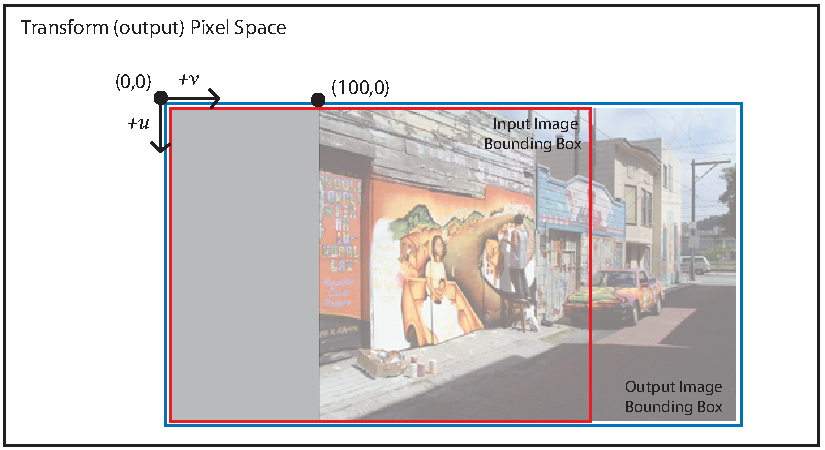
\includegraphics[width=5in]{images/transformed_mural.pdf}
\end{center}
  \caption{Using the {\tt crop()} function, you can select any region
    of the transformed (in this case, translated) image that you need.}
  \label{fig:transformed_mural}
\end{figure}

Note that the Vision Workbench adopts a consistent coordinate system
when working with pixels in the transformed image space.  The origin
is at the upper left hand corner of the original image, with the $u$
coordinate increases as you move down the rows of the image.  Figure
\ref{fig:transformed_mural} shows this coordinate system and the input
and output bounding boxes in the case of the the cropped, translated
image example we have been working with.

Using this intuition, we can now answer the second question posed
above.  When the pixels are translated off of the right edge of the
image, they disappear unless they are explicitly selected using
\verb#crop()#.  The only other reasonable behavior might have been to
have the pixels wrap around and enter on the left side of the image.
This is not supported using the Vision Workbench \verb#translate()#
function, however, as you will learn in the next section, such
transformations are still possible using the general transform
framework.

Finally, we arrive at the third question: what pixel value is used to
fill area where the original image has no data?  To answer this, think
back to the discussion of edge extension modes for the filter routines
in section \ref{sec:filter-edge-extend}.  Edge extension behavior in
the transform routines of the Vision Workbench are specified in an
identical fashion.

\begin{verbatim} 
  result_image = translate(input_image, 
                           u_translation, v_translation, 
                           ConstantEdgeExtension());
\end{verbatim}

In this example, the left 100x240 block of \verb#result_image# will contain
the ``smeared out'' pixels from the left side of the input image.  Of
course, this is probably not what you wanted, so the default behavior
edge extension behavior for \verb#translate()# is set to
\verb#ZeroEdgeExtension()#.

One final point before we move on to talking about image
transformations more generally.  Consider this block of code:

\begin{verbatim} 
  double u_transformations = 100.5;
  double v_transformation = 30.7;
  result_image = translate(input_image, u_translation, v_translation, 
                           ConstantEdgeExtension(), BicubicInterpolation());
\end{verbatim}

Here, the image is translated by a non-integer number of pixels.  This
is a totally reasonable thing to do, but it raises the question of how
one accesses a non-integer pixel location in the source image.  The
answer: interpolation.  As with edge extension, you can
specify the interpolation mode by passing in a dummy argument to the
\verb#translate()# function.  Table \ref{tbl:interpolation-modes}
shows the built-in interpolation types.

\begin{table}[t]\begin{centering}
\begin{tabular}{|c|l|l|} \hline
Type & Description \\ \hline \hline
\verb#NearestPixelInterpolation# & Use the nearest integer valued pixel location \\ \hline
\verb#Bilinear Interpolation# & Linearly interpolation based on the four nearest pixel values \\ \hline
\verb#Bicubic Interpolation# & Quadritic interpolation based on the nine nearest pixel values \\ \hline
\end{tabular}
\caption{The Vision Workbench Interpolation Modes.}
\label{tbl:interpolation-modes}
\end{centering}\end{table}

\subsection{Creating a New Transform}

Having now addressed some of the fundamental issues that arise when
transforming images, we now turn our discussion to how one might
formulate and implement a new image transformation algorithm.

In the most general sense, a transform is computed by performing the
following two steps for every pixel in the output image.

\begin{itemize}
\item Given the coordinates $X_{out}$ of a pixel in the output image,
  apply a transformation that yields the coordinates $X_{in}$ of a
  source pixel in the input image.  
\item Use some edge extension and interpolation scheme to determine
  the pixel value of the input image at $X_{in}$ (it may fall in
  between integer pixels coordinates or outside of the input image
  entirely) and set the value of the output image at $X_{out}$ to this
  value.
\end{itemize} 

When formulating a new image transformation algorithm, the first step
where all of the interesting work happens.  The code for interpolation
and edge extension is important, but usually incidental to the
transformation under development.  Ideally, one would focus
exclusively on writing code to perform the geometric calculations in
step one.  To help us with this task, we will introduce a new
programming idiom that appears commonly in the Vision Workbench: the
{\em functor}.

Technically, a functor is a C++ class that has implemented the
\verb#operator()# method.  Once created, such a class can be called
and passed around in place of a normal C++ function.  It behaves
identically except that, as a C++ object, the functor can maintain its
own state (possibly initialized when the functor is constructed).  In
the Vision Workbench, we use this definition more loosely to mean any
small function object that adheres to a small, pre-determined
interface.  But, rather than linger over semantic details, let's
jump straight to an example so that you can see what we mean.


\sourcelst{transform-functor.h}{An example transform functor that
  performs image translation.}

Let's look at the definition for the functor that describes image
translation, shown in Listing~\ref{lst:transform-functor.h}.  You'll
notice that this class has defined three methods: a constructor and
two methods called \verb#forward()# and \verb#reverse()#.  The class
also inherits from \verb#TransformBase<>#, but that's not something to
dwell on here.  For now just be aware that \verb#TransformBase<>#
provides default implementations that throw \verb#vw::UnimplErr()#
exceptions in case the subclass does not implement both methods.

The constructor is used to initialize the state of this functor; in
this case, an offset in x and y.  The \verb#reverse()# method is the
most important.  It performs step one in our list at the beginning of
this section.  Pretty simple, right?  Although the transformation in
this example is nothing special, the \verb#reverse()# method could
potentially be long and complicated.  So long as it returns a pixel
position in the input image in the end, we're happy.

The \verb#forward()# method performs the inverse operation of the
\verb#reverse()# method.  This method is not always necessary.  We'll
discuss it more in Section \ref{sec:transform-advanced-techniques}.

The beauty of the \verb#TranslateTransform# class, or any other class
that defines a set of \verb#forward()# and \verb#reverse()# methods is
that it can be passed as an argument to the \verb#transform()# function.

\begin{verbatim} 
  result_image = transform(input_image, 
                           TranslateTransform(u_translation, v_translation));
\end{verbatim}

This block of code performs the very same transformations as our call
to \verb#translate()# in the previous section.  (In fact,
\verb#translate()# is just a thin wrapper around \verb#transform()#
provided for convenience.)  As with the previous example, the edge
extend and interpolation modes can be supplied as dummy arguments to
\verb#transform()#.

As you can probably now see, the possibilities are endless!  For
example, we could also have used \verb#HomographyTransform# (another
built-in transform functor) to describe the same translation.  The
linear homogeneous transform that encodes a 100 pixel shift to the
right is:

\begin{equation}
H =
\left(
\begin{array}{ccc}
 1 & 0  & 100  \\
 0 & 1  & 0  \\
 0 & 0  & 1  
\end{array}
\right)
\end{equation}

Dropping the \verb#HomographyTransform# into \verb#transform()# yields
the same \verb#result_image# once again.

\begin{verbatim} 
  vw::Matrix<double> H = ... // defined as above
  result_image = transform(input_image, HomographyTransform(H));
\end{verbatim}

Any transform functor that adheres to this simple interface, including
one of your own devising, can be passed into \verb#transform#.  To
summarize, you can create and use your own transformation functor
\verb#foo# by following these steps.
\begin{itemize}
\item Inherit from \verb#public TransformBase<foo>#
\item Define a constructor that stores any state information that you need
\item Define a \verb#reverse()# method 
\item Define a \verb#forward()# method (optional, see Section \ref{sec:transform-advanced-techniques})
\end{itemize}

Of course, some of the most common transform functors are provided for
you as part of the Vision Workbench.  Refer to Table
\ref{tbl:transform-functors} for a list of built-in classes available
in \verb#<vw/Image/Transform.h>#

\begin{table}[tbh]\begin{centering}
\begin{tabular}{|c|l|l|} \hline
Type & Function & Description \\ \hline \hline
\verb#ResampleTransform# & \verb#resample()# & Scale an image, resizing the output image as needed \\ \hline
\verb#TranslateTransform# & \verb#translate()# & Translate an image \\ \hline
\verb#HomographyTransform# & & Apply a linear homogeneous transformation (3x3 Matrix)  \\ \hline
\verb#PointLookupTransform# & & Apply a transformation based on a lookup table image  \\ \hline
\verb#PointOffsetTransform# & & Apply a transformation based on an offset table image \\ \hline
\end{tabular}
\caption{Built-in transform functors and (if available) their function interface.}
\label{tbl:transform-functors}
\end{centering}\end{table}

\subsection{Advanced Techniques}
\label{sec:transform-advanced-techniques}

To wrap up our discussion of the transform methods, here are some
advanced techniques that you may find useful when working with image
transformations.

It is not uncommon to ask, for a given transform functor, what
bounding box in the transformed image space contains the complete set
of transformed pixels.  The \verb#compute_transformed_bbox()# routine
answers this question by performing the \verb#forward()#
transformation for each pixel location in the input image and growing
a bounding box to contain all of the forward transformed pixels.  This
bounding box can be passed directly as the second argument to
\verb#crop()#.

\begin{verbatim} 
  // Output image is cropped to contain all transformed pixels
  BBox2f result_bbox = compute_transformed_bbox(input_image, 
                                                MyTransformFunctor());
  result_image = crop(transform(input_image, MyTransformFunctor()),
                      result_bbox);
\end{verbatim}

For performance limited applications, you may find
\verb#compute_transformed_bbox_fast()# more appropriate.  It computes
the bounding box by applying \verb#forward()# to the perimeter pixels
of the input image only.  This should produce identical results to the
``slow'' version so long as the perimeter pixels of the input
image form the perimeter of the output image under the transformation
in question.

Finally, we would like to point out the existence of the
\verb#RadialTransformAdaptor# class.  This class is useful when it is
easier or more natural to describe a transformation in terms of polar
coordinates $[r,\theta]$ instead of the usual cartesian coordinates
$[u, v]$.

To use \verb#RadialTransformAdaptor#, you write your transform functor
as usual, but you interpret the components in the input and output
\verb#Vector2# to be $[r,\theta]$, in that order.  Assuming you have
created a class \verb#MyRadialTransform# in this manner, you can apply
it as follows:

\begin{verbatim} 
  result_image = transform(input_image, 
                           RadialTransformAdaptor(MyRadialTransform(),
                                                  input_image));
\end{verbatim}

The \verb#RadialTransformAdaptor# creates a polar coordinate system
wherein the center of the image is the origin, and a value of $r=1.0$ is
equal to the distance from the center to the left edge of the image.

\section{Pixel Mask}

At this point is best to introduce a new pixel type,
\verb#PixelMask#. It was convientantly hidden from the previous
chapter as it is not exactly just another pixel type. It does infact
though still have that same blue collar past of the others from
Table~\ref{tbl:pixel-types} and that means all operations the previous
Pixel types could do, \verb#PixelMask# can do as
well. \verb#PixelMask# just happens to append an additional boolean
channel value to what ever pixel type it encapsulates.

\begin{table}[h]\begin{centering}
\begin{tabular}{|c|l|l|} \hline
Type & Description & Channels \\ \hline \hline
\verb#PixelMask<PixelT<T> ># & Additional valid bit & One plus whatever \verb#PixelT# is \\ \hline
\end{tabular}
\caption{An addendum to standard Vision Workbench pixel types. {\tt PixelT} should generally be one of the types from Table~\ref{tbl:pixel-types} and {\tt T} should generally be from Table~\ref{tbl:channel-types}.}
\label{tbl:pixel-mask}
\end{centering}
\end{table}

This additional boolean channel is a pixel's validity. During FileIO
the boolean channel can correctly be interpreted as determining if a
pixel is transparent or not. This may seem as just a redundant binary
version of an alpha channel and it can correctly be interpreted as
this. Yet it has one ability that an alpha channel does not. The state
of a \verb#PixelMask# being invalid is quite like the 'T' virus from
\emph{Resident Evil} fame. It spreads to all other \verb#PixelMask#s
it is operated with. Meaning that given an image that has bad
pixels in it, they can be labelled as invalid and will remain so
through all operations.

A \verb#PixelMask# passes all of it access functions on to its inner
pixel type. So that a \verb#pixel[0]# will still return a red channel
from a pixel of type \verb#PixelMask<PixelRGB<float> >#. Yet remember
that it adds and an additional channel. So a \verb#PixelMask#'s
validity can be access with \verb#pixel[3]# or instead with a
\verb#pixel.valid()#.

Testing for a pixel's validity via a \verb#pixel.valid()# only works
if a pixel is a \verb#PixelMask#. But what if a function is written
generally for all pixels and it must test for a valid pixel like
\verb#blob_index#? In that case, Vision Workbench provides a series of
commands for working with a pixel validity despite the type. They are
listed in Table~\ref{tbl:pixel-mask-functions}.

\begin{table}[htb]\begin{centering}
\begin{tabular}{|c|l|} \hline
Function & Description \\ \hline \hline
\verb#is_transparent(PixelT)# & Tests if a pixel is transparent. In other words, not valid. \\ \hline
\verb#is_valid(PixelT)# & Tests as expected. \\ \hline
\verb#validate(PixelT)# & Forces a pixel valid \emph{iff} \verb#PixelMask#. Otherwise no-op. \\ \hline
\verb#invalidate(PixelT)# & Forces a pixel invalid \emph{iff} \verb#PixelMask# \\ \hline
\verb#toggle(PixelT)# & Changes the state of validity \emph{iff} \verb#PixelMask# \\ \hline
\verb#remove_mask(PixelT)# & Strips off the \verb#PixelMask# wrapper and returns the inner pixel type. \\ \hline
\end{tabular}
\caption{Pixel type safe functions for working with a {\tt PixelMask}'s valid bit.}
\label{tbl:pixel-mask-functions}
\end{centering}
\end{table}

Lastly, Vision Workbench provides a number of ImageView operators
working pixel validity. They are listed in
Table~\ref{tbl:pixel-mask-image-ops}.

\begin{table}[htb]\begin{centering}
\begin{tabular}{|c|p{5 in}|} \hline
Function & Description \\ \hline \hline
\verb#create_mask(im,s)# & Given a non \verb#PixelMask# view \verb#im#, returns an \verb#ImageView# of type \verb#PixelMask#. Pixels of valud \verb#s# are listed as invalid. \\ \hline 
\verb#create_mask(im,lo,hi)# & As previously, except \verb#lo# and \verb#hi# describe the valid pixel range. Pixels outside of that range are listed as invalid. \\ \hline
\verb#apply_mask(im,s)# & This removes the \verb#PixelMask# type, and replaces invalid pixels with a value \verb#s#. \\ \hline
\verb#copy_mask(im,mask)# & Copies an image \verb#mask#'s transparency on to an image \verb#im# of non-\verb#PixelMask# type. \\ \hline
\verb#mask_to_alpha(im)# & Convert a \verb#PixelMask# view to a view with a alpha channel. \\ \hline
\verb#edge_mask(im)# & Searches for the edges of an image and marks the first valid pixel, invalid. \\ \hline
\verb#invert_mask(im)# & Given an image of \verb#PixelMask#s , inverts every pixels validity. \\ \hline
\verb#validate_mask(im)# & Forces all pixels to be valid. \\ \hline
\verb#invalidate_mask(im)# & Forces all pixels to be invalid. \\ \hline
\verb#union_mask(im,mask)# & Unions the \verb#PixelMask# of \verb#mask# with \verb#im#, and keeping the image data in \verb#im#. \\ \hline
\verb#intersect_mask(im,mask)# & Intersects the \verb#PixelMask# of \verb#mask# with \verb#im#, and keeping the image data in \verb#im#. \\ \hline
\end{tabular}
\caption{Image operations for working with {\tt PixelMasks}}
\label{tbl:pixel-mask-image-ops}
\end{centering}
\end{table}

%% \section{Where to Go from Here}
